    \documentclass{minimal}
\usepackage{tikz}
\usetikzlibrary{trees}
\begin{document}
	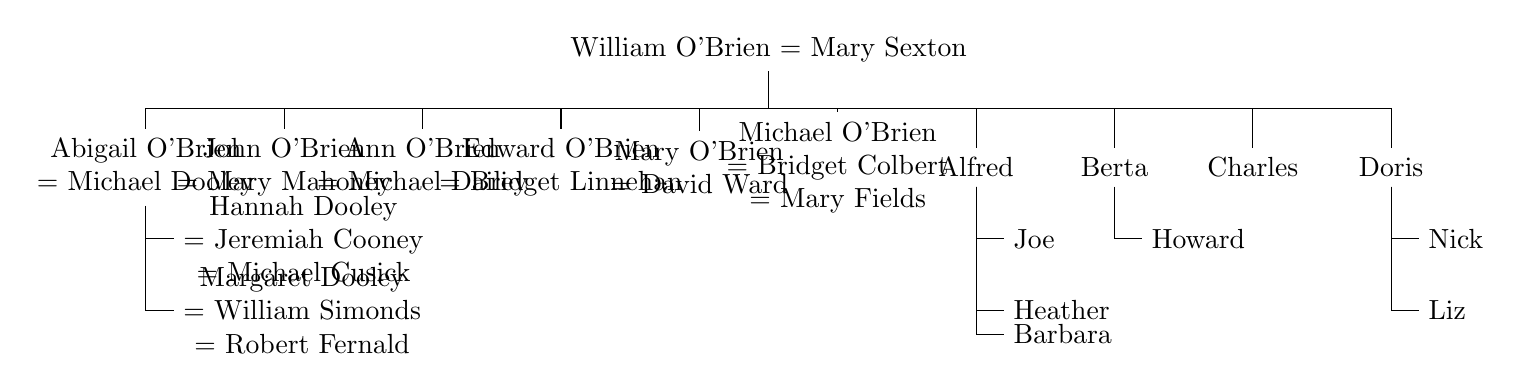
\begin{tikzpicture}[
	grandchild/.style={grow=down,xshift=1em,anchor=west,
		edge from parent path={(\tikzparentnode.south) |- (\tikzchildnode.west)}},
	first/.style={level distance=6ex},
	second/.style={level distance=12ex},
	third/.style={level distance=14ex},
	level 1/.style={sibling distance=5em},align=center]
	% Parents
	% \coordinate
	\node {William O'Brien = Mary Sexton}
	[edge from parent fork down]
	% Children and grandchildren
	child { node {Abigail O'Brien \\= Michael Dooley}
		child[grandchild,first] { node {Hannah Dooley \\= Jeremiah Cooney \\= Michael Cusick}}
		child[grandchild,second] { node {Margaret Dooley \\= William Simonds \\= Robert Fernald}} 
	}
	child { node {John O'Brien \\= Mary Mahoney}}
	child { node {Ann O'Brien \\= Michael Dailey}}
	child { node {Edward O'Brien \\= Bridget Linnehan}}
	child { node {Mary O'Brien \\= David Ward}}
	child { node {Michael O'Brien \\= Bridget Colbert \\= Mary Fields}}
	child{node{Alfred}
		child[grandchild,first] {node{Joe}}
		child[grandchild,second] {node{Heather}}
		child[grandchild,third] {node{Barbara}}}
	child{node{Berta}
		child[grandchild,first] {node{Howard}}}
	child {node{Charles}}
	child {node{Doris}
		child[grandchild,first] {node{Nick}}
		child[grandchild,second] {node{Liz}}};
	\end{tikzpicture}
\end{document}